\section{CAFE問題}\label{sec:background}

%-------------------------------------------------------
\begin{figure*}[t]
  \centering
  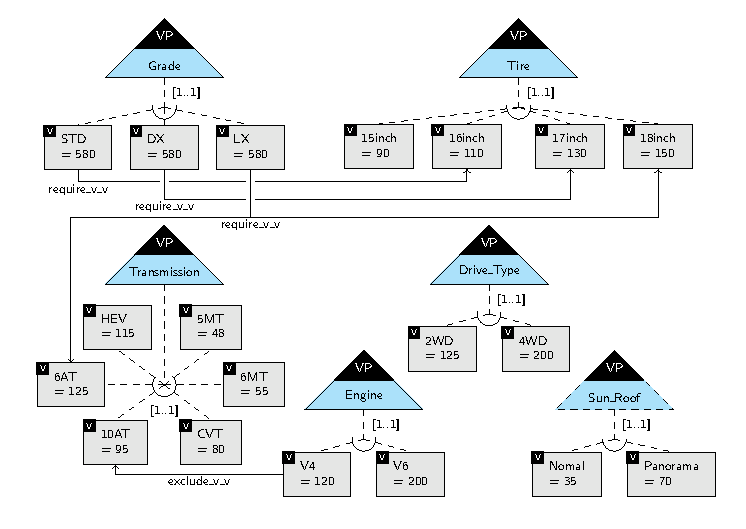
\includegraphics[width=0.8\linewidth]{images/ovm_example.eps}
  \caption{CAFE問題の例}
  \label{fig:ovm_example}
\end{figure*}
%-------------------------------------------------------

CAFE問題の入力は以下の通りである.
以降,
装備タイプをタイプ,
装備オプションをオプション
と簡単に書くことにする.
\begin{enumerate}
\item タイプの集合\label{input:vp}
\item オプションの集合\label{input:v}
\item タイプとオプションの対応関係\label{input:vp-v}
\item 各タイプで選択可能なオプション数の上下限値\label{input:ublb}
\item タイプ同士,オプション同士,および,タイプとオプション間の依存関係
  \label{input:dependency}
\item 各オプションに付加された IWR 値\label{input:iwr}
%%%
\item 求めたい装備仕様の個数\label{input:g}
\item 各装備仕様とタイプ(あるいはオプション)間の依存関係\label{input:init}
\item 各装備仕様に含まれるオプションの IWR 値の総和と燃費との対応表\label{input:fe}
\item 各装備仕様に含まれるオプションの IWR 値の総和と予想販売台数との対応表\label{input:sv}
\item CAFE 基準値\label{input:cafe}
\end{enumerate}
入力~\ref{input:iwr}の IWR は Inertial Working Rating の略で,
直観的には各オプションの重量を表す.
入力~\ref{input:g}の個数は,求めたい派生車両の数と考えるとわかりやすい.
CAFE問題は,上記の入力から,
装備および燃費に関する制約を満たしつつ,
予想販売台数を最大化する車両装備仕様を求める問題である.

CAFE問題の制約は以下の通りである.
\begin{description}
\item[範囲制約]: 各装備仕様について,各タイプで選択されるオプション数は,
  入力~\ref{input:ublb}で与えられた上下限値の範囲内でなければならない.
\item[依存制約]: 各装備仕様について,入力~\ref{input:dependency}で与
  えられた依存関係を満たさなければならない.
  依存制約には,要求制約と排他制約の2つがある.
\item[燃費制約]: 入力~\ref{input:cafe}の CAFE 基準値を$t$,
  入力~\ref{input:g}の装備仕様個数を$n$として,
  以下の CAFE 規制を満たさなければならない.
  \begin{adjustvboxheight}
  \[
    \begin{array}{lcr}
      & & \\
      \displaystyle\frac{\sum_{i=1}^{n} FE_{i}\cdot SV_{i}}{\sum_{i=1}^{n} SV_{i}}
      &
        \geq 
      &
        t \\
      & & 
    \end{array}
  \]
  \end{adjustvboxheight}
  不等式の左辺は$n$個の装備仕様の\textbf{平均燃費}を表している.
  $FE_{i}$と$SV_{i}$は,装備仕様$i$の燃費と予想販売台数を表しており,
  それぞれ,入力~\ref{input:fe}と\ref{input:sv}の対応表を元に計算される.
\item[初期制約]:
  入力~\ref{input:init}で与えられた依存関係を満たさなければならない.
\end{description}

%%%%%%%%%%%%%%%%%%%%%%%%%%%%
%-------------------------------------------------------
\begin{figure}[tb]
  \centering
  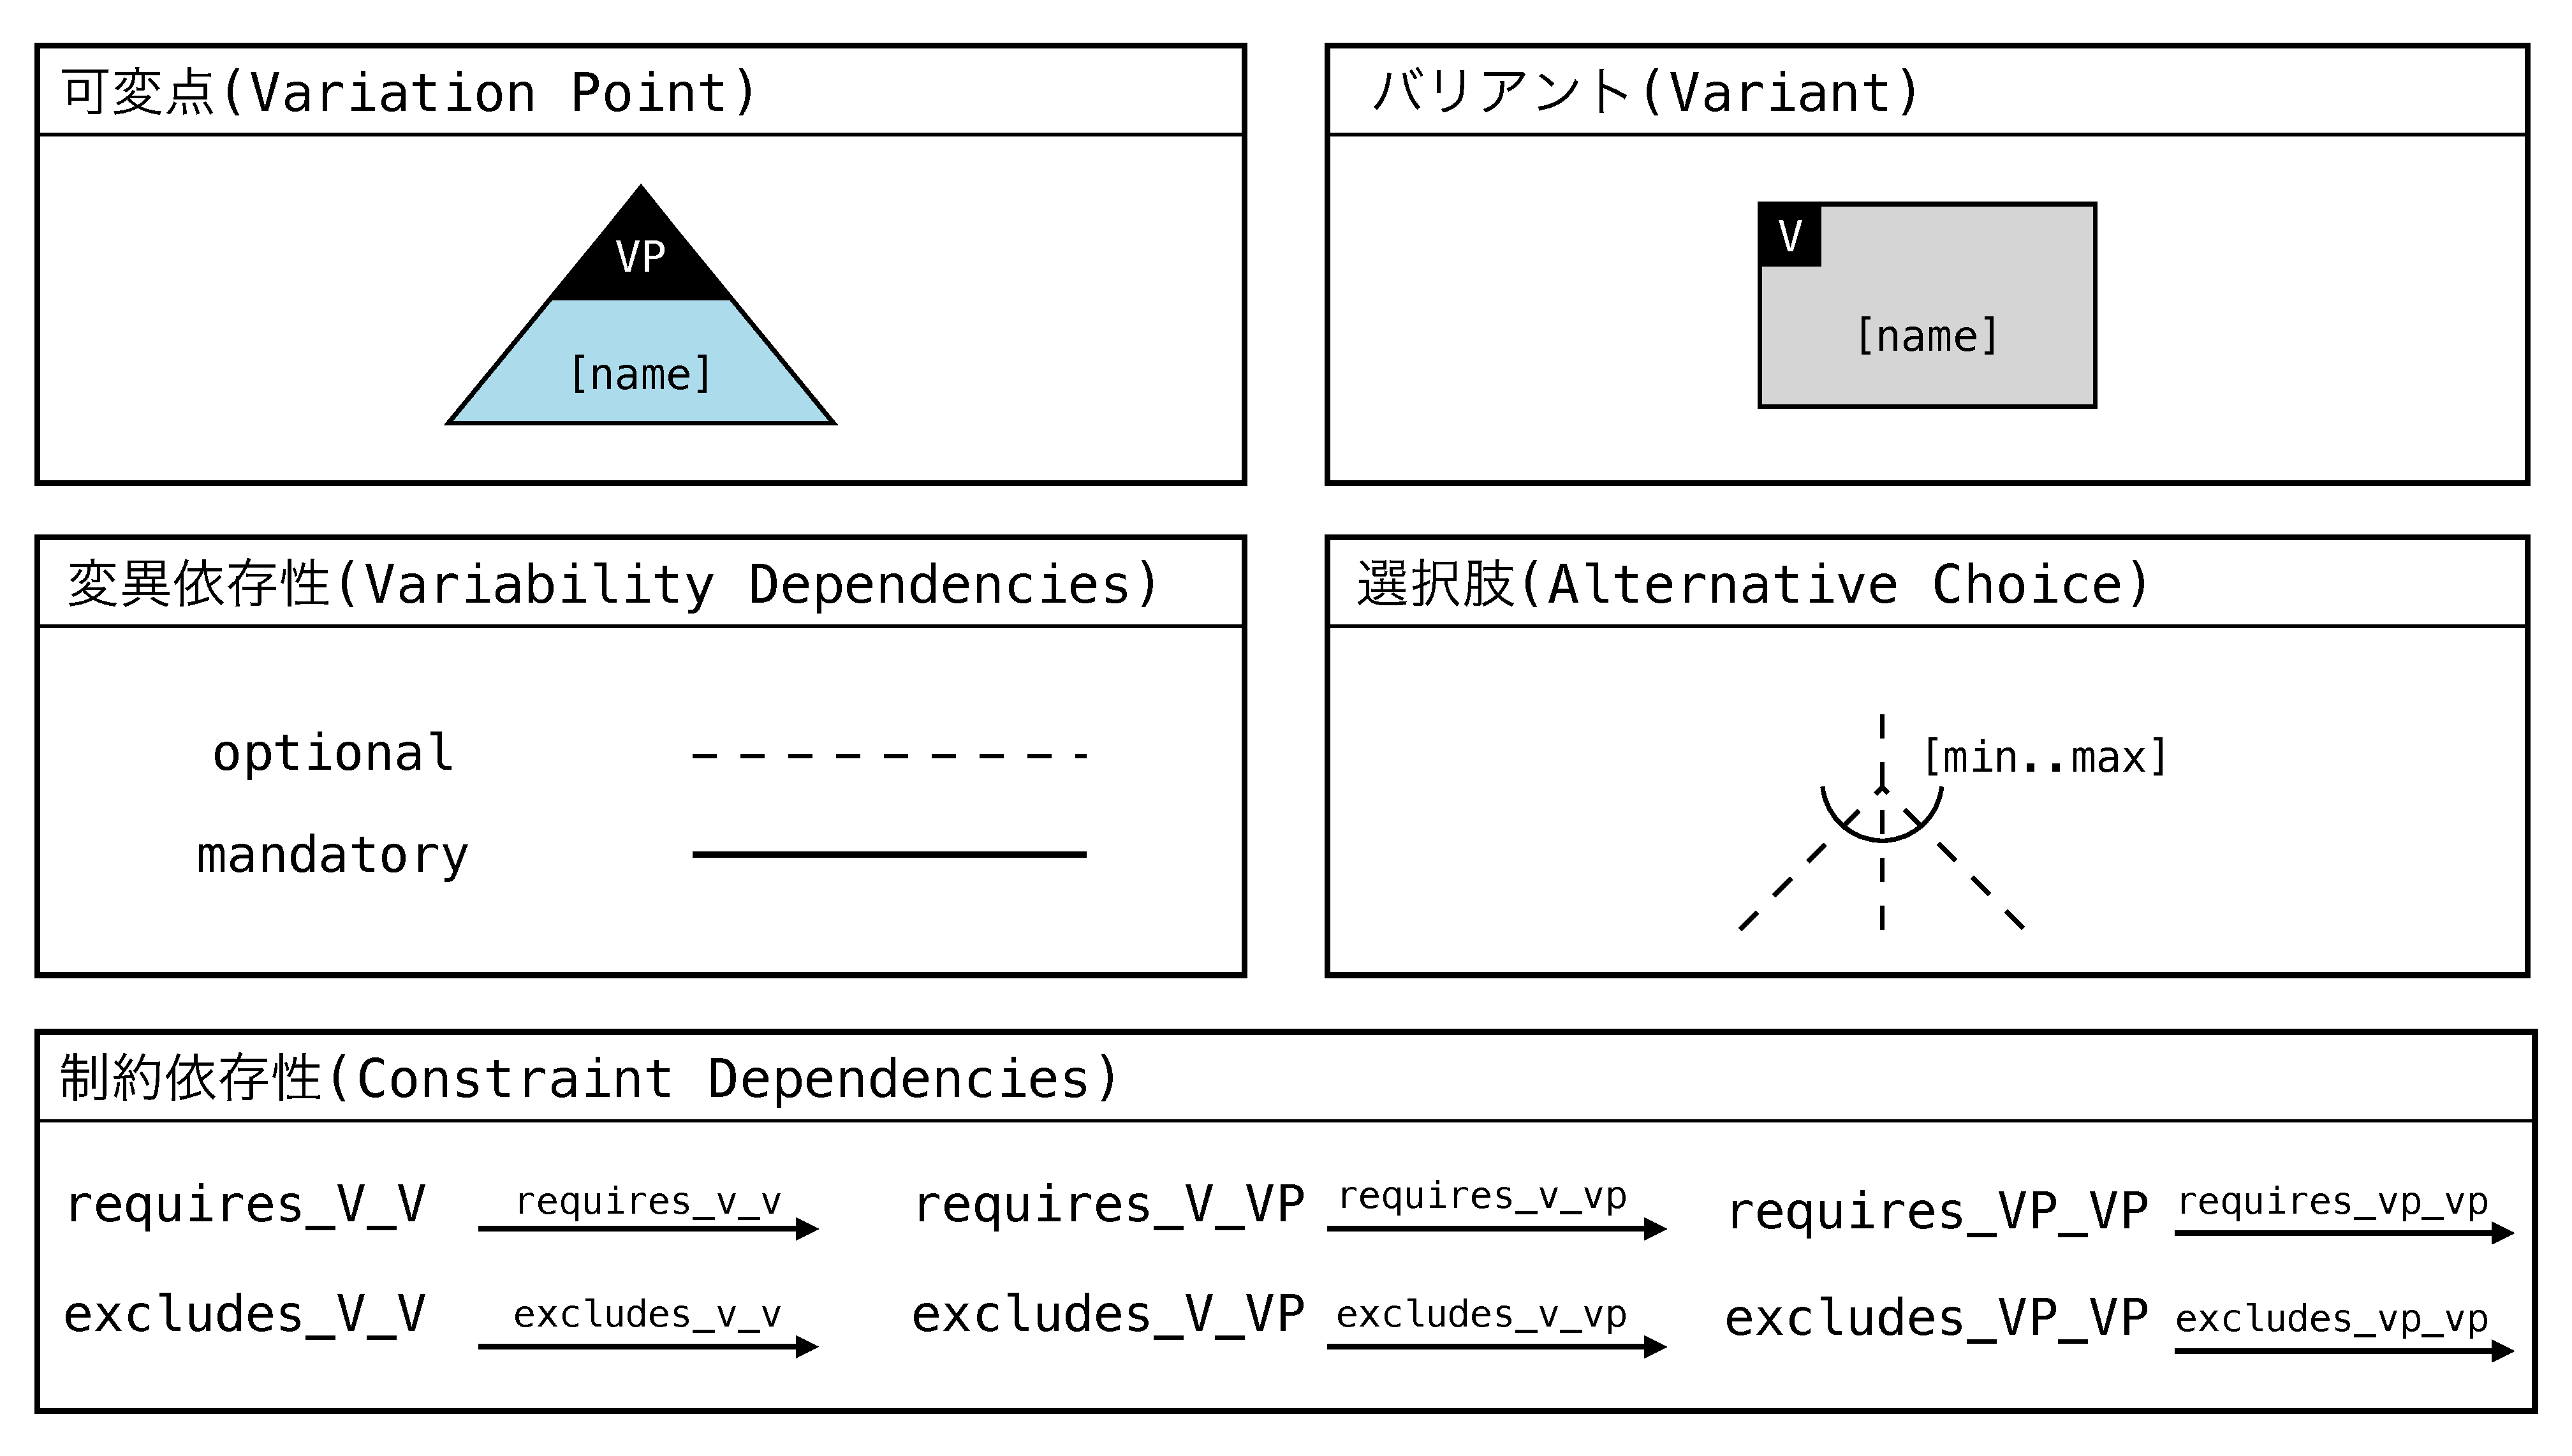
\includegraphics[width=\linewidth]{images/notation.eps}
  \caption{可変性モデルの表記法\cite{Pohl05:sple}}
  \label{fig:ovm_notation}
\end{figure}
%-------------------------------------------------------

CAFE問題の例を図~\ref{fig:ovm_example}に示す.
この例は,ソフトウェアプロダクトライン開発の分野で用いられる
\textbf{可変性モデル} (Orthogonal Variability Model; OVM\cite{Pohl05:sple})
によって記述されている.
図~\ref{fig:ovm_notation}に,可変性モデルの基本的な表記法を示す.
可変性モデルでは,
仕様ごとに変わりうる項目を\textbf{可変点}と呼び,三角形で表す.
可変点の具体的なインスタンスを\textbf{バリアント}と呼び,長方形で表す.
可変点とバリアントの対応関係には\textbf{変異依存性}と\textbf{選択肢}があり,
選択肢の場合は,その多重度も付記される.
可変点同士,バリアント同士,および,可変点とバリアント間の依存関係は,
\textbf{制約依存性}によって表される.
制約依存性には,要求(\textsf{requires})と排除(\textsf{excludes})の2種類がある.

可変性モデルでCAFE問題を記述する場合,
タイプは可変点,
オプションとその IWR 値はバリアント,
タイプとオプションの対応関係および
選択可能なオプション数の上下限値は選択肢,
タイプ同士,オプション同士,および,タイプとオプション間の依存関係は
制約依存性によって表される.
以上から,CAFE問題の入力のうち,
\ref{input:vp}〜\ref{input:iwr}は可変性モデルによって記述されるこ
とがわかる.

図~\ref{fig:ovm_example}の問題例は,
6個のタイプ,19個のオプション,5個の依存制約から構成され,
各タイプの選択可能なオプション数はすべて1である.
本論文では,可変点で表されるタイプは,各装備仕様に対して必須とする.
ただし,\textsf{Sun\_Roof}のような選択可能なタイプ(必須ではないタイプ)
については,破線の可変点で表すものとする.

%-------------------------------------------------------
\begin{table}[t]
  \centering
  \caption{CAFE問題(図~\ref{fig:ovm_example})の解}
  \begin{tabular}{l|l|c|c|c} \bhline
    %\multicolumn{1}{c|}{装備}   & \multicolumn{3}{c}{装備仕様} \\ \cline{2-4}
    \multicolumn{2}{l|}{装備仕様}               & 1	& 2 	 & 3	\\  \hline
    装備 & \textsf{Grade}        & \textsf{STD}    & \textsf{DX}     & \textsf{LX}\\
    &\textsf{Drive\_Type}  & \textsf{2WD}    & \textsf{2WD}    & \textsf{2WD}\\
    &\textsf{Engine}	  & \textsf{V4}     & \textsf{V6}     & \textsf{V6}\\
    &\textsf{Tire}	  & \textsf{16inch} & \textsf{17inch} & \textsf{18inch}\\
    &\textsf{Transmission} & \textsf{5MT}    & \textsf{6MT}    & \textsf{10AT}\\
    &\textsf{Sun\_Roof}    & -               & \textsf{Normal} & -  \\ \hline
    \multicolumn{2}{l|}{IWR 値の総和}           & 983  & 1,125   & 1,180 \\ %\hline
    \multicolumn{2}{l|}{燃費(km/L)}      & 10.2  & 8.9     & 8.5 \\ %\hline
    \multicolumn{2}{l|}{予想販売台数}    & 745   & 1,988   & 1,171  \\ \hline
    \multicolumn{2}{l|}{平均燃費(km/L)}  & \multicolumn{3}{c}{9.0} \\ 
    \multicolumn{2}{l|}{予想販売台数(合計)}  & \multicolumn{3}{c}{3,904} \\ \hline
 \end{tabular}
 \label{tab:ovm_ans}
\end{table}
%-------------------------------------------------------

図~\ref{fig:ovm_example}の問題に対する解の例を表\ref{tab:ovm_ans}に示す.
この解は,
CAFE 基準値に9.0km/L,
求めたい装備仕様の個数に3を与え,
装備仕様とオプションの依存関係として,
(装備仕様1, \textsf{STD}),
(装備仕様2, \textsf{DX}),
(装備仕様3, \textsf{LX})
を要求して得られたものである.
各装備仕様の燃費(km/L)は,左から順に 10.2, 8.9, 8.5 と
個々には CAFE 基準値を満たしていないが,
3台の平均燃費は 9.028km/L となり,CAFE 規制を満たしている.


%%% Local Variables:
%%% mode: japanese-latex
%%% TeX-master: "paper"
%%% End:
